\documentclass[conference]{IEEEtran}
\usepackage{graphicx}
\usepackage{url}
\usepackage{listings}
\usepackage{color}

\definecolor{codegray}{gray}{0.95}
\lstset{
  backgroundcolor=\color{codegray},
  basicstyle=\ttfamily\small,
  frame=single,
  breaklines=true,
  columns=fullflexible
}

\begin{document}

\title{Thera-Hand Mechanical Instructions}
\author{\IEEEauthorblockN{Andy Vo, Ethan Cesario, Aliyaa Islam}
\IEEEauthorblockA{Department of Computer Science and Engineering\\
University of California, Santa Cruz}}
\maketitle

\section{ESP32-C3 Setup Instructions}

This section describes how to configure the ESP32-C3 development board for use on a personal computer.

\subsection{Requirements}
\begin{itemize}
    \item ESP32-C3 development board
    \item USB-C cable
    \item Internet-enabled computer (Windows, Linux, or macOS)
    \item Git
    \item Python 3.7 or later
\end{itemize}

\subsection{Installation of Prerequisites}

\subsubsection{Python}
Download and install Python from \url{https://www.python.org/downloads/}. During installation, ensure the option to add Python to the system PATH is selected.

\subsubsection{Git}
Download Git from \url{https://git-scm.com/} and complete the installation using default settings.

\subsection{ESP-IDF Installation}

To install the official Espressif IoT Development Framework (ESP-IDF), execute the following commands:

\begin{lstlisting}
git clone --recursive https://github.com/espressif/esp-idf.git
cd esp-idf
\end{lstlisting}

Then run the install script:

\begin{itemize}
    \item Linux/macOS:
    \begin{lstlisting}
    ./install.sh
    \end{lstlisting}
    \item Windows:
    \begin{lstlisting}
    install.bat
    \end{lstlisting}
\end{itemize}

\subsection{Environment Setup}

Before building or flashing firmware, set up the environment as follows:

\begin{itemize}
    \item Linux/macOS:
    \begin{lstlisting}
    . ./export.sh
    \end{lstlisting}
    \item Windows:
    \begin{lstlisting}
    export.bat
    \end{lstlisting}
\end{itemize}

\subsection{Flashing and Testing}

Connect the ESP32-C3 board to the computer via USB. Identify the correct serial port:

\begin{itemize}
    \item Linux/macOS: \texttt{ls /dev/ttyUSB*} or \texttt{ls /dev/cu.*}
    \item Windows: Use Device Manager to find the COM port
\end{itemize}

Build and flash a project using:

\begin{lstlisting}
idf.py build
idf.py -p [PORT] flash
idf.py -p [PORT] monitor
\end{lstlisting}

Replace \texttt{[PORT]} with the detected port name.

\subsection{Troubleshooting}
\begin{itemize}
    \item Ensure drivers for USB-to-UART chips (e.g., CP210x, CH340) are installed.
    \item Use a data-capable USB cable.
    \item If the board does not respond, reset it using the \texttt{EN} button and retry.
\end{itemize}

\section{Wiring Instructions for Flex Sensors and Servos}

This section explains how to wire five flex sensors and two Smraza Micro Servo S51 motors to the ESP32-C3 using a breadboard. Refer to Fig.~\ref{fig:circuit} for a visual representation.

\subsection{Flex Sensor Connections}

Each of the five flex sensors is connected in a voltage divider configuration using a 10~k$\Omega$ pull-down resistor. The resulting analog voltage can be read by the ESP32-C3.

\begin{itemize}
    \item One end of each flex sensor connects to the 3.3~V power rail.
    \item The other end of each sensor connects to a GPIO pin and a 10~k$\Omega$ resistor.
    \item Each 10~k$\Omega$ resistor is connected to ground (GND).
    \item The junction between the sensor and resistor is connected to the ESP32-C3 ADC input pins as follows:
    \begin{itemize}
        \item Sensor 0 $\rightarrow$ GPIO0
        \item Sensor 1 $\rightarrow$ GPIO1
        \item Sensor 2 $\rightarrow$ GPIO2
        \item Sensor 3 $\rightarrow$ GPIO3
        \item Sensor 4 $\rightarrow$ GPIO4
    \end{itemize}
\end{itemize}

\subsection{Servo Motor Connections}

Two Smraza Micro Servo S51 motors are connected to the ESP32-C3:

\begin{itemize}
    \item \textbf{Power:} Connect the red (V\textsubscript{CC}) wire of each servo to the 5~V power rail.
    \item \textbf{Ground:} Connect the brown/black (GND) wire of each servo to the ground rail.
    \item \textbf{Signal:} Connect the yellow/white signal wires to the GPIO pins:
    \begin{itemize}
        \item Servo 0 $\rightarrow$ GPIO5
        \item Servo 1 $\rightarrow$ GPIO7
    \end{itemize}
\end{itemize}

\begin{figure}[!ht]
    \centering
    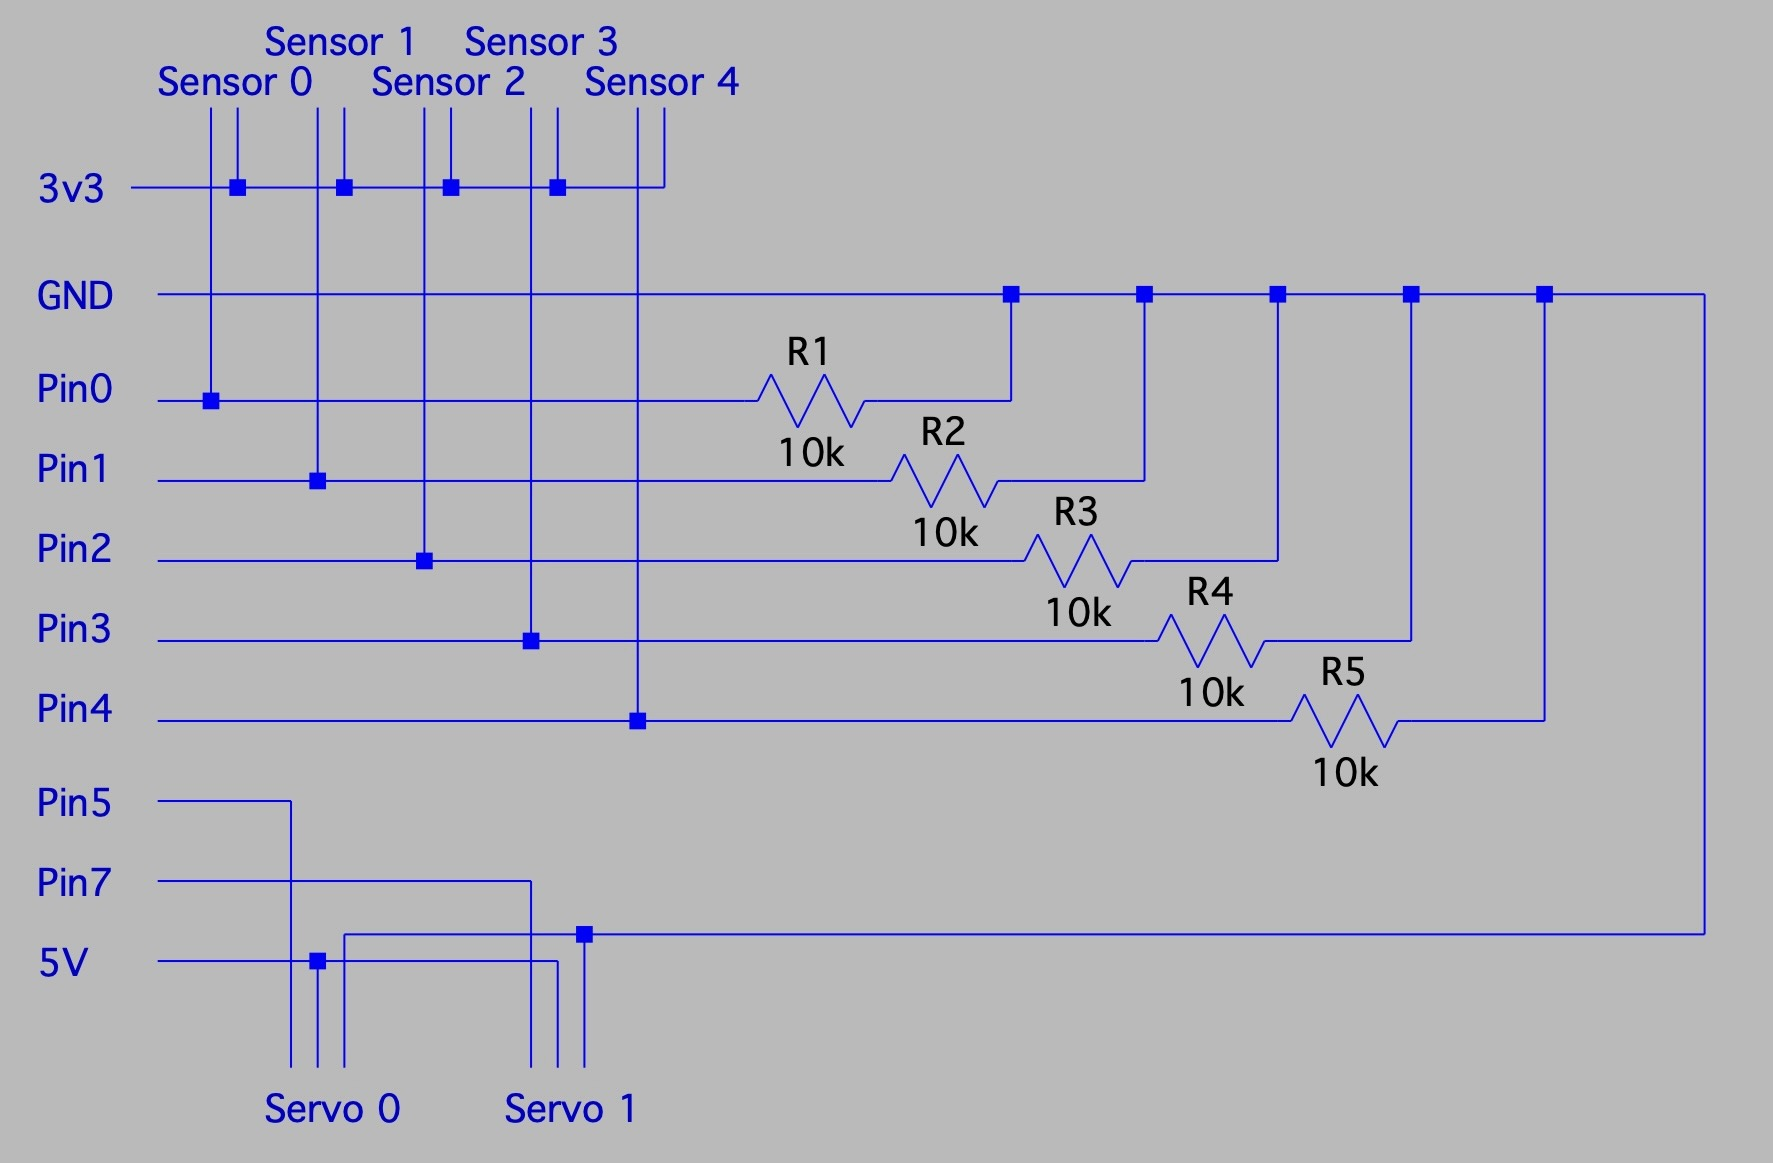
\includegraphics[width=0.45\textwidth]{proto1.jpeg}
    \caption{Circuit diagram showing ESP32-C3 wiring with 5 flex sensors and 2 Smraza Micro Servo S51 motors.}
    \label{fig:circuit}
\end{figure}

\section{Functional Testing and Calibration}

After wiring the ESP32-C3 with the flex sensors and servos as described in the previous section, functionality can be verified using two test scripts: one for the flex sensors and another for servo motion.

\subsection{Flex Sensor Data Capture}

A Python or C-based script is used to read the analog values from the ESP32-C3's ADC pins. These values are mapped linearly to a range of 0 to 100. Based on empirical testing, flex sensor states are interpreted as follows:

\begin{itemize}
    \item Values $\leq 40$: Sensor is bent \textbf{backwards}
    \item Values $> 40$: Sensor is bent \textbf{forwards}
\end{itemize}

These thresholds can be fine-tuned per sensor using calibration profiles stored in software.

\subsection{Servo Function Testing}

A separate script drives the two Smraza Micro Servo S51 motors through their full range of motion for two minutes. The test parameters are as follows:

\begin{itemize}
    \item \textbf{Waveform Generator:} Squarewave, 50~Hz frequency, 5~V\textsubscript{PP} (peak-to-peak)
    \item \textbf{Power Supply:} 4.8~V, 5~A
    \item \textbf{PWM Duty Cycle Calibration:}
    \begin{itemize}
        \item \textbf{2.3\% duty cycle:} Servo rotates fully to the \textbf{left}
        \item \textbf{12.4\% duty cycle:} Servo rotates fully to the \textbf{right}
    \end{itemize}
\end{itemize}

These values are used to validate the full operational range of the servo motors and ensure consistent response to PWM control signals.

\textit{Note: Although many hobby servos accept 3.3~V control signals, some may require signal level shifting to 5~V for reliable operation.}

\section{5V Power Supply and Continuous Servo Control}

To power two Parallax continuous rotation servos simultaneously, a regulated 5~V power supply is connected via a barrel jack interface. This setup provides adequate current and voltage stability to operate both servos under load.

\subsection{Barrel Jack Power Setup}

\begin{itemize}
    \item Use a 5~V DC power supply rated at a minimum of 2~A.
    \item Connect the positive terminal of the power supply to the barrel jack's center pin.
    \item Connect the ground terminal to the outer sleeve of the barrel jack.
    \item The barrel jack then connects to the breadboard's 5~V and GND rails.
    \item From the breadboard rails, connect power and ground to each Parallax servo as follows:
    \begin{itemize}
        \item Red wire (V\textsubscript{CC}) $\rightarrow$ 5~V rail
        \item Black wire (GND) $\rightarrow$ GND rail
        \item White wire (signal) $\rightarrow$ ESP32-C3 GPIO pin
    \end{itemize}
    \item Example GPIO assignments:
    \begin{itemize}
        \item Servo A $\rightarrow$ GPIO6
        \item Servo B $\rightarrow$ GPIO7
    \end{itemize}
\end{itemize}

\subsection{Servo Direction Test Program}

A test script is used to validate bidirectional rotation of both continuous rotation servos. The following logic is applied:

\begin{itemize}
    \item Rotate both servos clockwise for 20 seconds.
    \item Pause momentarily.
    \item Rotate both servos counter-clockwise for 20 seconds.
\end{itemize}

The direction of rotation is determined by the PWM duty cycle:

\begin{itemize}
    \item \textbf{Clockwise:} 1.3~ms pulse width (approximately 6.5\% duty at 50~Hz)
    \item \textbf{Counter-clockwise:} 1.7~ms pulse width (approximately 8.5\% duty at 50~Hz)
    \item \textbf{Stop (optional):} 1.5~ms pulse width (neutral)
\end{itemize}

An example pseudocode implementation:

\begin{lstlisting}
    // Pseudocode for testing Parallax servos
    setPWMFrequency(50);  // 50 Hz standard
    setPWMDuty(GPIO6, 6.5);  // Clockwise
    setPWMDuty(GPIO7, 6.5);
    delay(20000);  // 20 seconds

    setPWMDuty(GPIO6, 8.5);  // Counter-clockwise
    setPWMDuty(GPIO7, 8.5);
    delay(20000);  // 20 seconds

    // Optionally stop
    setPWMDuty(GPIO6, 7.5);
    setPWMDuty(GPIO7, 7.5);
\end{lstlisting}

\subsection{Safety Notes}
\begin{itemize}
    \item Always power the ESP32-C3 from a separate 3.3~V source or USB while driving high-current loads like servos from 5~V.
    \item Verify power supply ratings and ensure the total current draw does not exceed 5~A.
    \item Add a common ground between all components (ESP32, servos, sensors, and power supply).
\end{itemize}

\end{document}